% \documentclass{book}

\documentclass[12pt]{article}
\usepackage[pdfborder={0 0 0.5 [3 2]}]{hyperref}%
\usepackage[left=1in,right=1in,top=1in,bottom=1in]{geometry}%
\usepackage[shortalphabetic]{amsrefs}%
\usepackage{amsmath}
\usepackage{enumerate}
\usepackage{enumitem}
\usepackage{amssymb}                
\usepackage{amsmath}                
\usepackage{amsfonts}
\usepackage{amsthm}
\usepackage{bbm}
\usepackage[table,xcdraw]{xcolor}
\usepackage{tikz}
\usepackage{float}
\usepackage{booktabs}
\usepackage{svg}
\usepackage{mathtools}
\usepackage{cool}
\usepackage{url}
\usepackage{graphicx,epsfig}
\usepackage{makecell}
\usepackage{array}

\def\noi{\noindent}
\def\T{{\mathbb T}}
\def\R{{\mathbb R}}
\def\N{{\mathbb N}}
\def\C{{\mathbb C}}
\def\Z{{\mathbb Z}}
\def\P{{\mathbb P}}
\def\E{{\mathbb E}}
\def\Q{\mathbb{Q}}
\def\ind{{\mathbb I}}

\graphicspath{ {images6/} }

\begin{document}
\section*{20 Feb 2017}
Now that we can construct the correct family of double pulses, we return to the regular 5th order KdV equation. For now, we use finite difference operators with Neumann boundary conditions. Continuation code is used until we reach speed of $c = 6.2755$. We look at the second pulse, which is the first one to have all eigenvalues on (or near) the imaginary axis. Idea is to look at exponentially weighted spaces, which will move the essential spectrum out of the way, and to see what is left.

\subsection*{Exponentially weighted spaces}
Through trial and error, we select 0.0001 as our exponential weight. First, we choose grid size $N = 10000$ and domain size $L = 100$. Linearizing about the second double pulse and using eigs, we get the eigenvalues closest to 0.

\begin{figure}[H]
\includegraphics[width=8.5cm]{eigs1.eps}
\includegraphics[width=8.5cm]{eigs1zoom.eps}
\end{figure}

The essential spectrum has successfully been moved to the right, and it takes the shape we expect. Note that we see a pair of complex conjugate eigenvalues which are to the right of the imaginary axis. There are three other eigenvalues on the real axis near 0 which are not part of the essential spectrum. For all three eigenvalues, a plot of the corresponding eigenfunction looks like (a scalar multiple of) the derivative of the double pulse. We show these three eigenfunctions below, together with a plot of the derivative of the double pulse.

\begin{figure}[H]
\includegraphics[width=8.5cm]{eig1fn1.eps}
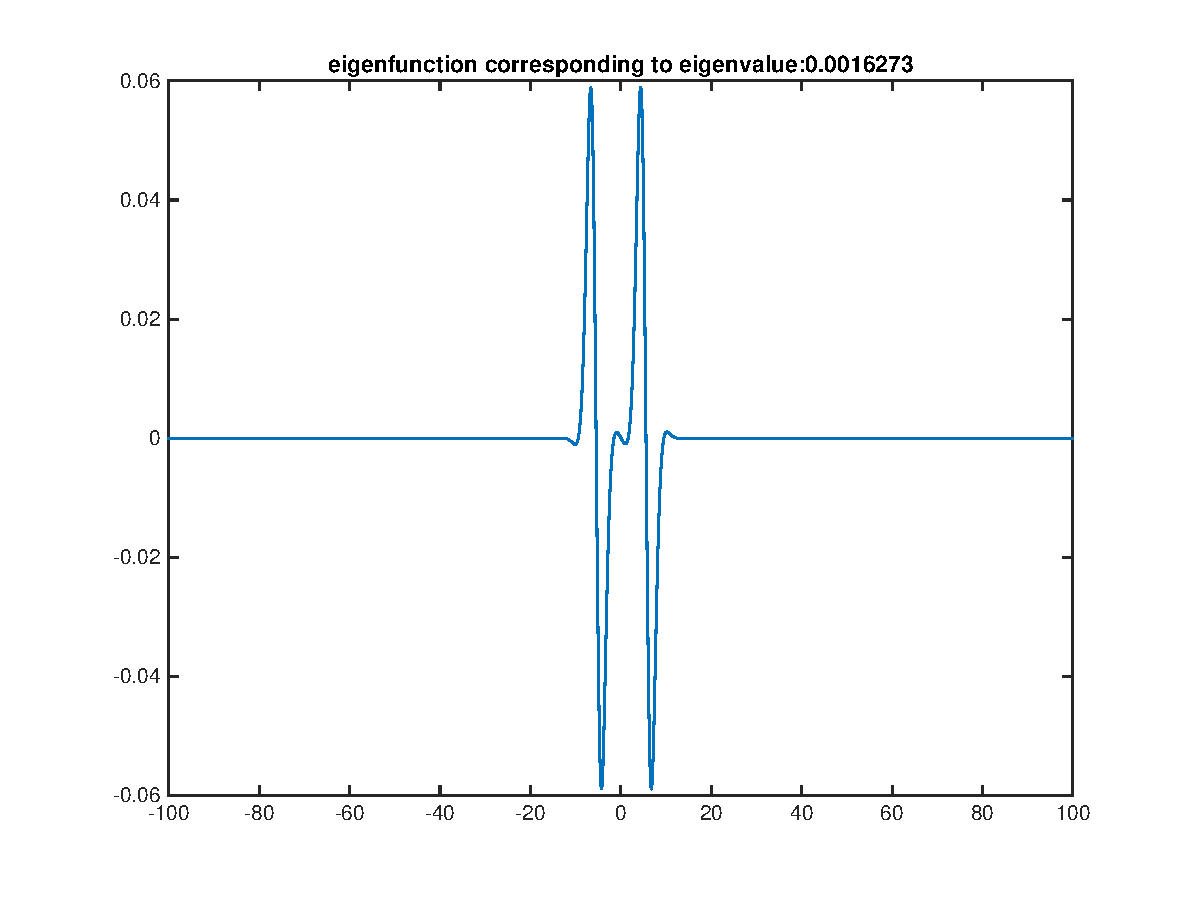
\includegraphics[width=8.5cm]{eig1fn2.eps}
\end{figure}
\begin{figure}[H]
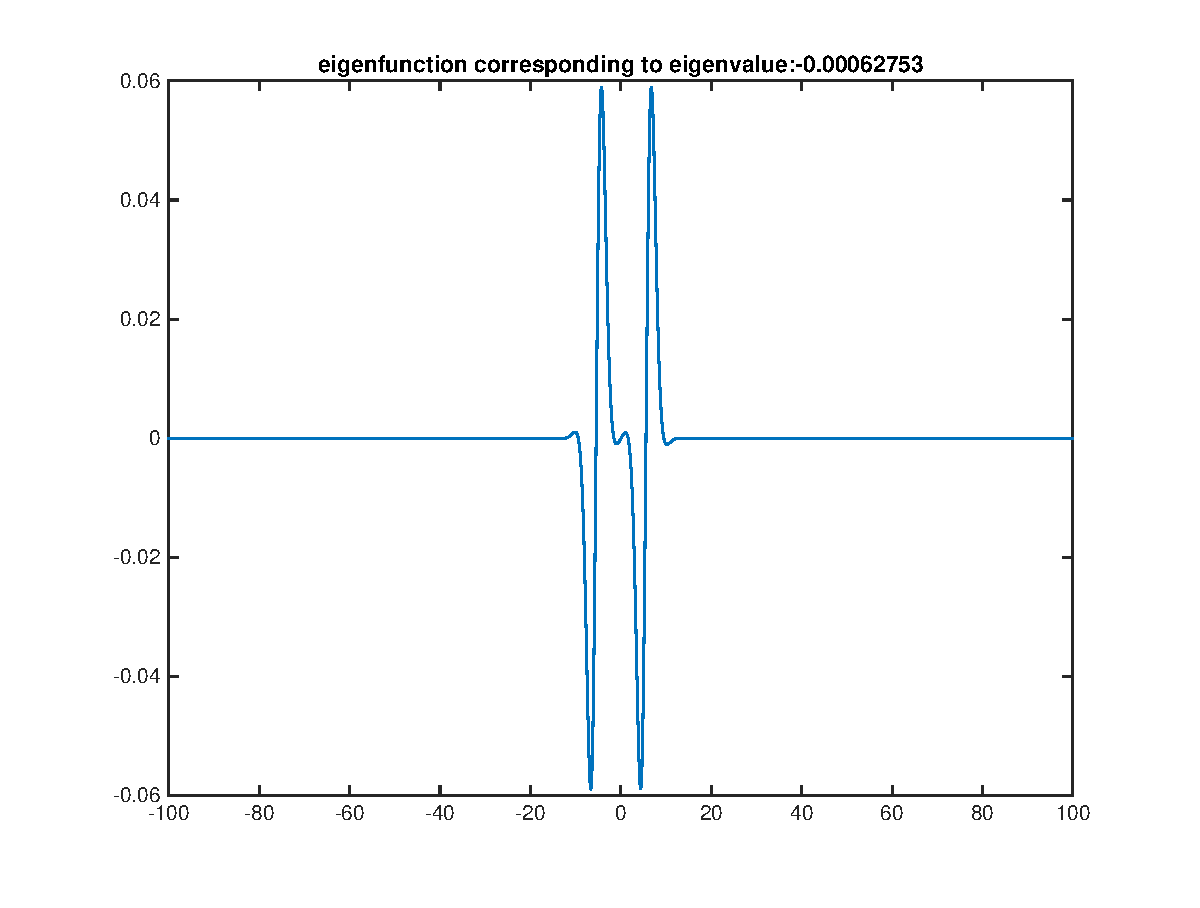
\includegraphics[width=8.5cm]{eig1fn3.eps}
\includegraphics[width=8.5cm]{d1deriv.eps}
\end{figure}

If we use different grid sizes, the complex conjugate pair of eigenvalues stay essentially put, whereas the other eigenvalues move around. Their corresponding eigenfunctions (or the real part, if they are complex) continues to look like the derivative of the double pulse. Here are zooms of the eigenvalues near 0 for $N = 5000, 20000, 50000$.

\begin{figure}[H]
\includegraphics[width=8.5cm]{eigs1zoom2.eps}
\includegraphics[width=8.5cm]{eigs1zoom3.eps}
\end{figure}
\begin{figure}[H]
\includegraphics[width=8.5cm]{eigs1zoom4.eps}
\end{figure}

I suspect that these eigenvalues should all really be 0, and the deviation from 0 is caused by error in the numerical method. This idea is further supported by the fact that these eigenvalues move around (but without pattern) as $N$ and $L$ are varied, but in all cases the corresponding eigenfunctions look like the derivative. Thus I think we can focus on the complex conjugate pair of eigenvalues.\\

Plotting the corresponding eigenfunctions, we see that the eigenfunctions are localized around 0, which is good.
\begin{figure}[H]
\includegraphics[width=8.5cm]{eigs1real.eps}
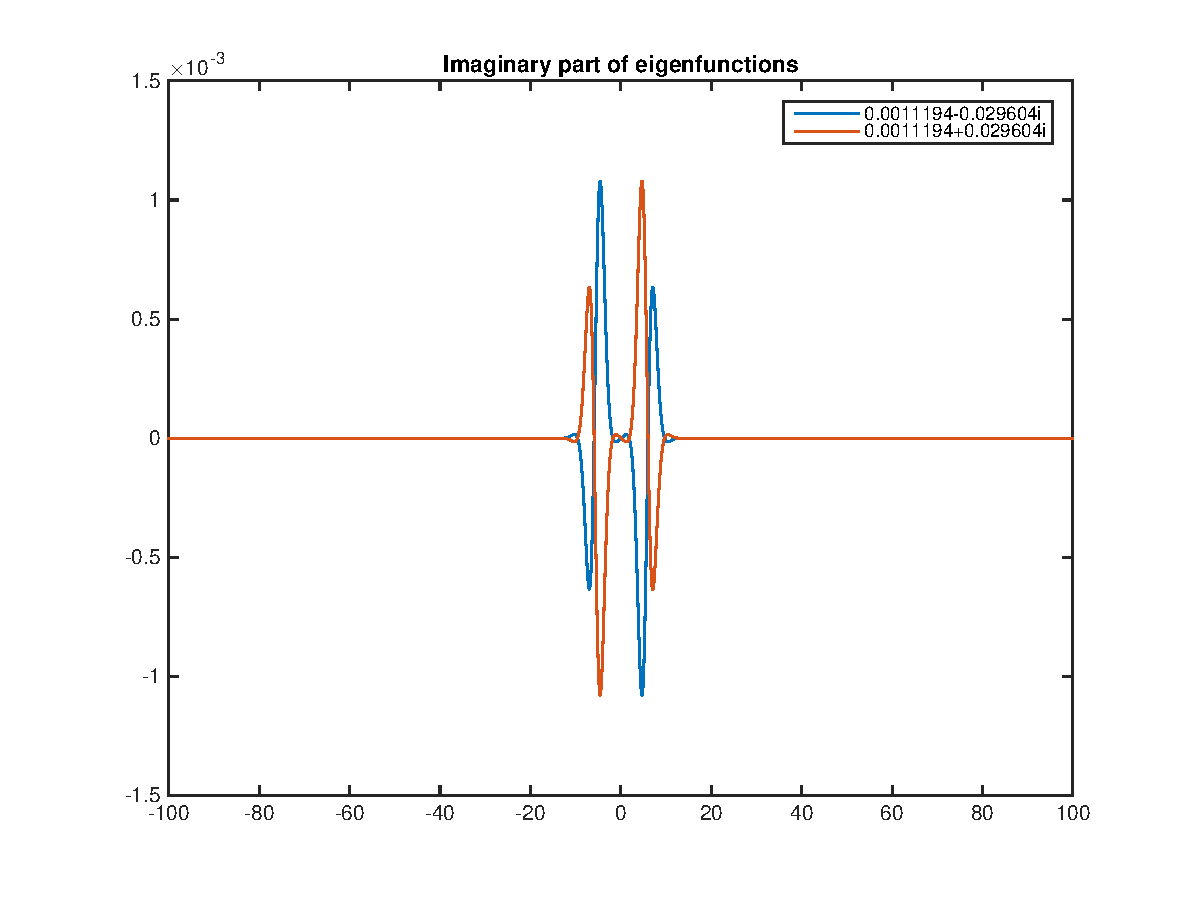
\includegraphics[width=8.5cm]{eigs1imag.eps}
\end{figure}


\subsection*{Experiment with grid and domain size}
First, we increase number of grid points.
\begin{figure}[H]
\begin{tabular}{l|l|l}
Grid size (N) & Domain length(L) & Eigenvalue pair near 0  \\ \hline
1000 &  50 & $0.0011 \pm 0.0280i$   \\
2000 &  50 & $0.0011 \pm 0.0295i$   \\
4000 &  50 & $0.0011 \pm 0.0296i$   \\
8000 &  50 & $0.0011 \pm 0.0296i$   \\
16000 & 60 & $0.0011 \pm 0.0295i$
\end{tabular}
\end{figure}
Essentially no change in eigenvalues, especially in real part. Next, increase domain length, keep mesh size constant, i.e. if we double domain length we also have to double grid size.
\begin{figure}[H]
\begin{tabular}{l|l|l}
Grid size (N) & Domain length(L) & Eigenvalue pair near 0  \\ \hline
2000 &  100 & $0.0011 \pm 0.0280i$ \\
4000 &  200 & $0.0011 \pm 0.0280i$ \\
8000 &  400 & $0.0011 \pm 0.0280i$ \\
16000&  800 & $0.0011 \pm 0.0280i$ \\
32000& 1600 & $0.0011 \pm 0.0280i$ \\
\end{tabular}
\end{figure}
If we take an extreme example (N = 10000, L = 2000), we still get $\lambda = 0.0011 \pm 0.0295i$, so the real part is essentially unchanged. Since with increasing numerical accuracy and domain size, the real part of this eigenvalue pair is not moving towards the imaginary axis, I think that for this double pulse (and thus for the similar ones) we have a quadruplet of eigenvalues.


\subsection*{Unexpected Eigenvalues}
So we expect two eigenvalues near 0, but we have three. This is weird, and not sure where they are coming from. To check and see whether the problem is with our numerical scheme or code, we repeat the same thing for the single pulse with known solution ($c =  0.2130$). Nothing is run through the fsolve. Domain size is $L = 100$. For finite difference methods, we have mesh size $N = 5000$, and for Fourier spectral methods we have $N = 2048$. 
Using the linearization about the known solution in an exponentially weighted space, we plot the eigenvalues for each method.

\begin{figure}[H]
\includegraphics[width=8.5cm]{knownsingleeigs.eps}
\includegraphics[width=8.5cm]{knownsingleeigszoom.eps}
\end{figure}

\begin{figure}[H]
\includegraphics[width=8.5cm]{knownsingleeigsfourier.eps}
\includegraphics[width=8.5cm]{knownsingleeigszoomfourier.eps}
\end{figure}

In all cases, the eigenfunctions (or real parts thereof) of the eigenvalues near 0 look like the derivative of the single pulse. For Fourier, we have a an extra eigenvalue near 0 and for finite difference we have an extra complex-conjugate pair of eigenvalues near 0. Not sure what to make of this.
\end{document}

